% Lab Writeup for Diode-Laser Spectroscopy Lab
% Adam Reyes, George Wong
% Advanced Lab FAll 2013


\documentclass[paper=a4, fontsize=11pt]{scrartcl} % A4 paper and 11pt font size
\usepackage[left=2.5cm,top=2.5cm,right=2.5cm,bottom=2.5cm]{geometry} 
\usepackage{amsmath}
\usepackage{graphicx}
\usepackage{sectsty}
\usepackage{fancyhdr}
\pagestyle{fancyplain}
\usepackage{subcaption}
\usepackage{wrapfig}
\usepackage[english]{babel}
\usepackage{float}

\numberwithin{equation}{section}
\numberwithin{figure}{section} 
\numberwithin{table}{section}
%\setlength\parindent{0pt}

\fancyhead[R]{\thepage} 
\fancyhead[L]{Reyes, Wong} 
\fancyhead[C]{Saturated Absorption Spectroscopy} 
\fancyfoot[L]{} 
\fancyfoot[C]{} 
\fancyfoot[R]{} 

\newcommand{\horrule}[1]{\rule{\linewidth}{#1}}

\title{	
Saturated Absorption Spectroscopy of Rubidium
\horrule{0.5pt}
\normalfont \normalsize 
\textsc{Advanced Experimental Physics }
}

\author{Adam Reyes \\ George Wong} % Your name

\date{\normalsize\today} % Today's date or a custom date


\begin{document}
\maketitle



%%%%%%%%%Abstract%%%%%%%%%%%%%%%%%%%%%
\textbf{Abstract:}
A diode-laser swept through the absorption bands of Rubidium was used
to measure the absorption spectrum of the Rubidium lines. With the use
of a pump beam, the saturated absorption of Rubidium was found and
used to investigate the fine structure of Rubidium. 

%%%%%%%%%%Introduction%%%%%%%%%%%%%%%%%%%%%
\section{Introduction}

\subsection{Doppler Broadening}

In general for any given monatomic gas there are atoms moving in all
directions with different speeds that follow some Poisson
distribution. From quantum mechanics we know that these atoms will
absorb photons only of particular frequencies. From only this
consideration, if we were to sweep some laser source through
these ``resonant'' frequencies we would expect sharp lines at
exactly these frequencies. 

We now consider the motion of the atoms
in some gas only along the direction of our laser. In the rest frame
of these atoms, if the atom is moving, it will experience a shift in
frequency of the incident photon, either increasing or decreasing
depending on the direction of motion. It is now easy to imagine, since we have
Poisson distribution of velocities, even off resonance some atoms will
experience a shift of the incident frequency towards resonance. In
effect this broadens the absorption lines we have previously
discussed. Figure~\ref{fig:broadening} shows a typical trace with Doppler broadening.

\begin{figure}[H] \begin{center}
  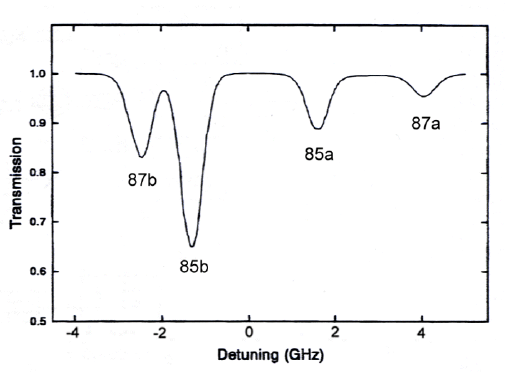
\includegraphics[height=60mm]{broadening.png}
  \caption{\textbf{Standard example of spectrum with Doppler broadening}}
  \label{fig:broadening}
\end{center} \end{figure}


\subsection{Saturated Absorption}

We now consider the same system of a monatomic gas that demonstrates
Doppler Broadening, but now have two collinear beams incident on the
gas in opposite directions. One of the beams is to have an intensity
much greater than the other, called the ``pump beam''. The weaker beam
is the one whose intensity will be measured, called the ``probe
beam''.

Off resonance only one beam can be shifted towards resonance for a
given atom since they are in opposite directions. As such in these
areas we expect the introduction of the second beam to have no impact
on the absorption spectrum and we would observe the same broadened
spectrum discussed in 1.1. 

We now consider those atoms which are at rest along the direction of
the beams. Since they are stationary with respect to the direction of
the beams there is no frequency shift for either beam. If the laser is
now exactly on resonance, since the pump has much greater intensity it
will saturate those stationary atoms in the excited state and cause
the probe to pass through, not being absorbed by the atoms along its
path. So at a particular resonance, when we are exactly on it, we
would expect a sharp peak in the absorption. 

It is also known from quantum mechanics that relativistic
considerations of an atomic electron leads to perturbations in its
Hamiltonian, such as through the coupling of its spin with its
motion. These perturbations lead to splitting of its ground state
energy levels, called the atom's fine structure. With this in mind, the saturated absorption spectrum of
our monatomic gas should have multiple sharp peaks within a larger
Doppler broadened peak. Figure~\ref{fig:hyperfine} shows this splitting.

\begin{figure}[H] \begin{center}
  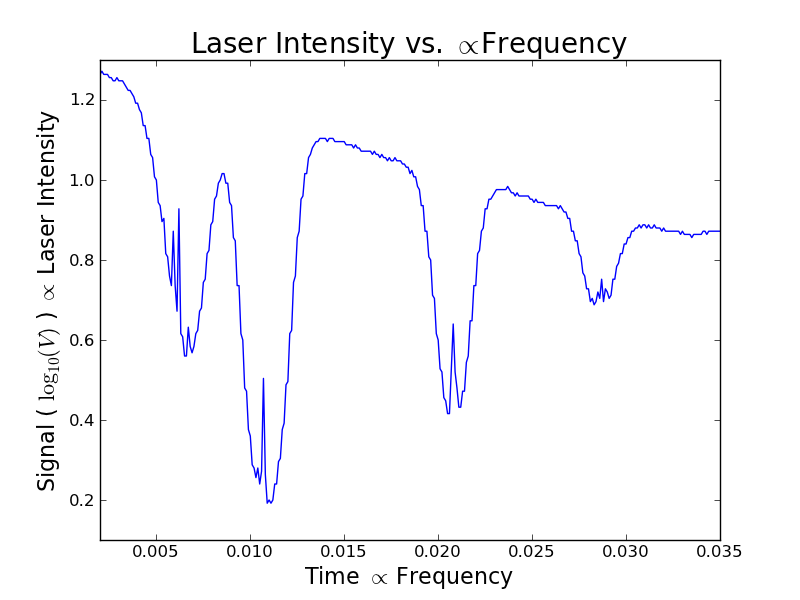
\includegraphics[height=100mm]{3-1-001.png}
  \caption{\textbf{Hyperfine splitting} as observed with the experimental set up used for this examination (sample shows intensity from combination of pump and probe beams). }
  \label{fig:absorb1}
\end{center} \end{figure}



%%%%%%%%%%%%%Methods%%%%%%%%%%%%%%%%%
\section{Methods}

\begin{figure}[H] \begin{center}
  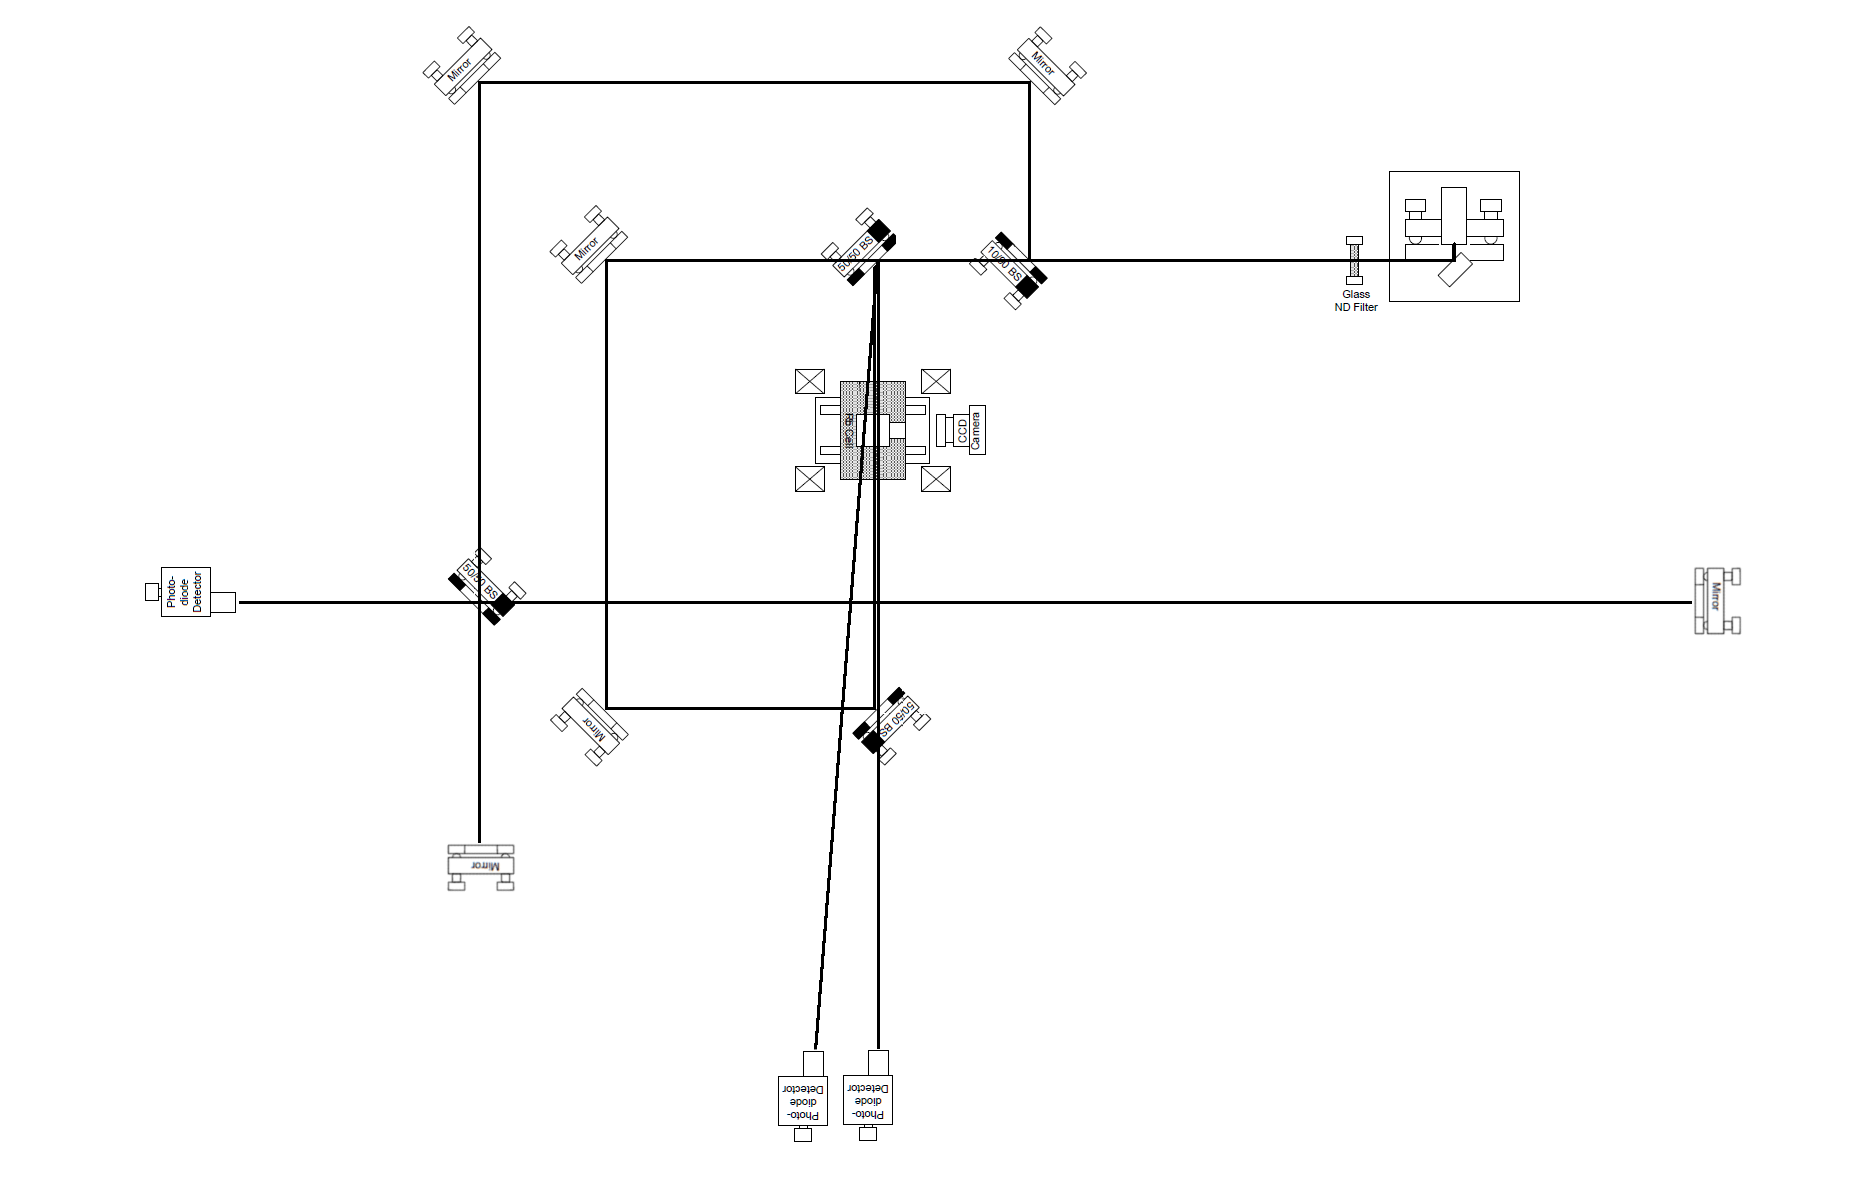
\includegraphics[height=80mm]{full.png}
  \caption{\textbf{Overall final set up of apparatus} showing placement of all beam splitters, mirrors, and various other devices. }
  \label{fig:absorb1}
\end{center} \end{figure}

\subsection{Absorption Spectrum}
The first part of the experiment was to observe the absorption spectrum of the Rubidium gas. By shining a laser directly through a chamber full of Rb gas and varying the frequency of the laser light, the rubidium gas would absorb those photons whose frequency matched the energy gap of electrons in the gas. This absorption would cause a drop in intensity of the passing beam in addition to causing florescence in the tube.

\begin{enumerate}
\item The provided laser was turned on (heated up) and the incident current amplitude was increased until the point where it was ``lasing''. See Figure~\ref{fig:lase}.
\item The laser was aimed at and through the Rb gas chamber.
\item A ramp voltage was applied to the piezoelectric within the laser assembly. This voltage controlled the frequency of vibration in a mirror placed in the laser's path. The changing frequency effectively allowed for changes in laser light frequency.
\item A CCTV camera, capable of viewing infrared light was aimed as the Rb gas chamber. The incident current to the laser assembly was increased until florescence was seen.
\item A photoelectric diode, capable of reporting incoming light intensity in the form of voltage, was placed in the path of the beam after it went through the chamber.
\item The voltage from the diode was measured on an oscilloscope against ramp voltage ($\propto$ frequency).
\item The voltage offset, frequency, and slope of the ramp were adjusted, as was the current to the laser. This was done until the absorption spectrum of both the $^{85}$Rb and $^{87}$Rb isotopes could be seen on the scope.
\item Several samples of the spectrum were taken. They are reproduced in Figures~\ref{fig:absorb1}$-$\ref{fig:absorb2}.
\item The voltage from the diode was then subtracted from the voltage of the ramp, with the scales of the two appropriately adjusted for compatibility. This allowed for observation of the spectrum without the ramp voltage artifact.
\end{enumerate}

\begin{figure}[H] \begin{center}
  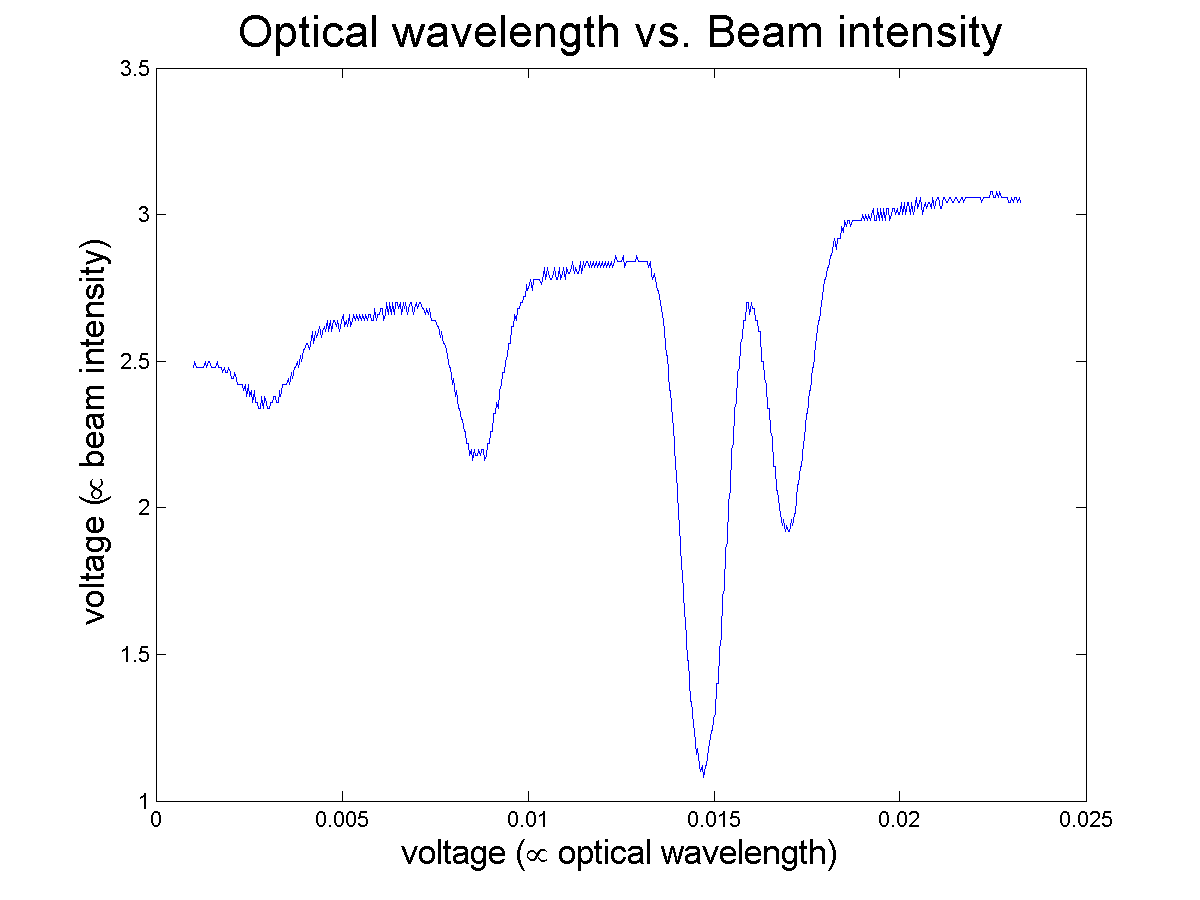
\includegraphics[height=80mm]{absorb3.png}
  \caption{\textbf{Intensity of Laser Beam with Varied Frequency through Rubidium Chamber} showing the effective absorption spectrum of Rubidium as a function of frequency (represented here as change in frequency over time). Here, signal (voltage) is modified by a ramp which adds a bias.}
  \label{fig:absorb1}
\end{center} \end{figure}

\begin{figure}[H] \begin{center}
  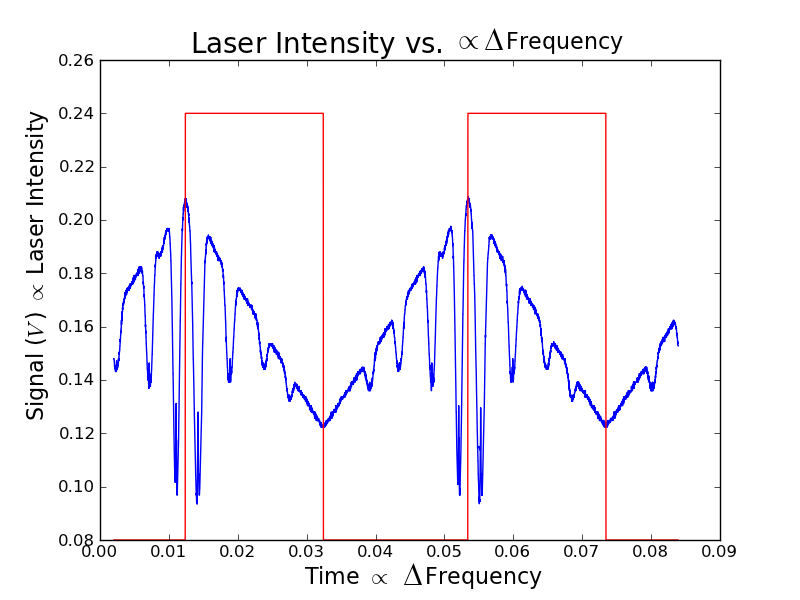
\includegraphics[height=80mm]{2-2-002.png}
  \caption{\textbf{Intensity of Laser Beam vs. Varying Laser Frequency with Pump}  shown over the course of approximately two full cycles in frequency.}
  \label{fig:absorb2}
\end{center} \end{figure}


\subsection{Pump Beam}
While the above method may be fine for viewing general absorption spectrum, due to Doppler broadening, many of the fine details are lost. To combat this, a new ``pump'' beam, at the same frequency and (preferably) from the same source is added in such a way that both the original (``probe'') beam and the pump beam overlap.

\begin{enumerate}
\item The original incident beam to the Rb chamber was split in two (using a 50-50 beam splitter) and one of the beams was directed around the chamber.
\item The beam directed around the chamber was aimed at another 50-50 beam splitter that reflected light back into the chamber.
\item The two beams that were passing through the chamber were aligned precisely at two points (as far away from each other as possible).
\item A ``wedge'' was placed in the path of the original beam entering the Rb chamber. Its purpose was to split the initial beam so that the difference in intensities for the pump+probe beam and only-probe beam could be detected.
\item The pump+probe beam was subtracted form the only-probe beam (with gains appropriately adjusted) and several data samples were taken. These data are reproduced in Figures~\ref{fig:withPump_1} and \ref{fig:withPump_2}.
\end{enumerate}


\begin{figure}[H] \begin{center}
  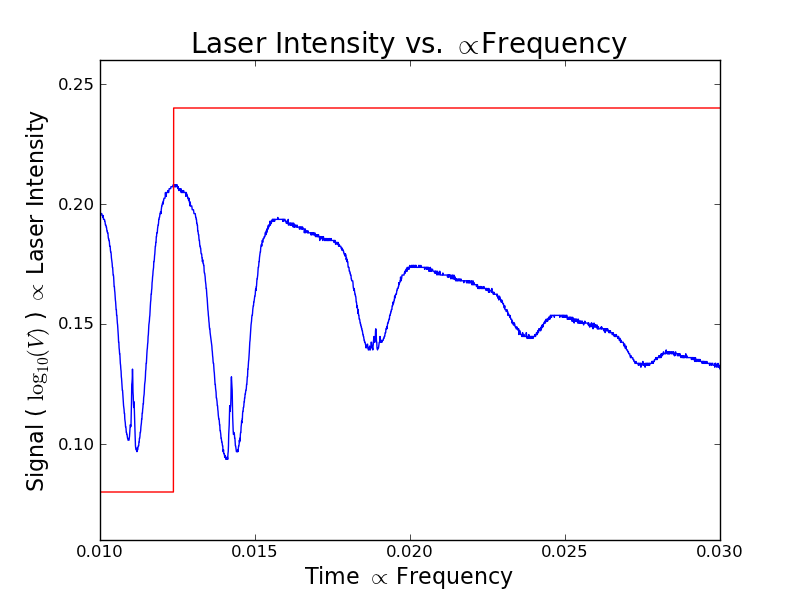
\includegraphics[height=80mm]{2-2-002-zoom.png}
  \caption{\textbf{Intensity of Laser Beam vs. Varying Laser Frequency with Pump} shown over a restricted interval. A Pump beam has clearly been added, as hyperfine splitting is more easily observable. }
  \label{fig:withPump_1}
\end{center} \end{figure}


\begin{figure}[H] \begin{center}
  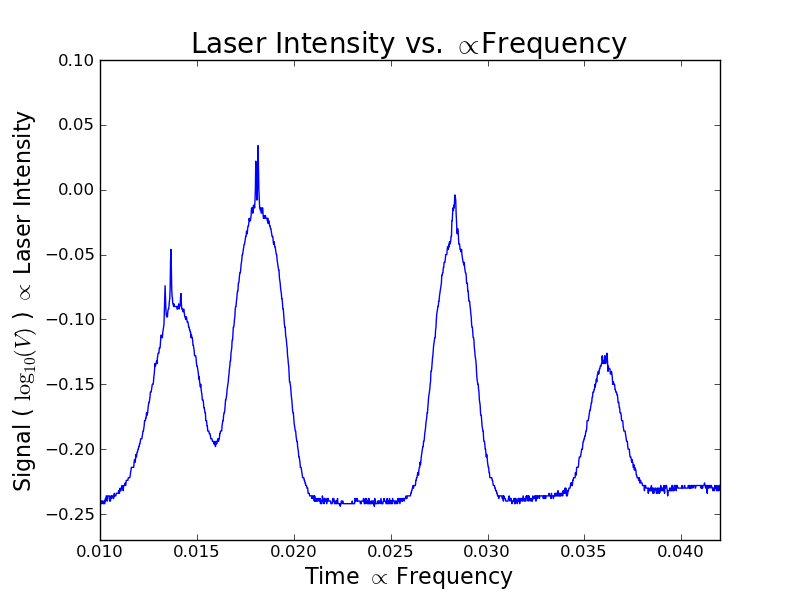
\includegraphics[height=80mm]{3-1-002.png}
  \caption{\textbf{Intensity of Laser Beam vs. Varying Laser Frequency with Pump} wherein the ramp has been subtracted from Figure~\ref{fig:withPump_1} to obtain a more useable/readable plot. Note that the dependent axis is in a logarithmic scale for visual purposes. }
  \label{fig:withPump_2}
\end{center} \end{figure}

\subsection{Interferometer}
To gain any meaningful \emph{numerical} data from the taken measurements, an idea of how to relate time / ramp voltage to frequency shift is necessary. One such way is to create an interferometer which allows for recording of changes in frequency by comparing path lengths. Beams traveling different lengths then recombined with constructively/destructively interfere with changes in wavelength. A set difference in path length will produce ``fringes'' with a sweep in frequency. \\

For a Michelson Interferometer the detected intensity goes as follows
\begin{equation}
I \propto 1 + cos\frac{4\pi \Delta Lf}{c}
\end{equation}
Where $\Delta L$ is the path length difference, $f$ is the frequency
and $c$ the speed of light. For a given fringe spacing $T$ there must
be a corresponding shift in frequency $\delta f$. Using the previous
expression this is given as
\begin{equation}
\delta f = \frac{c}{2\Delta L T}
\end{equation}
From this a change in frequency can be calculated from an oscilloscope
trace of the interferometer by finding the fringe spacing and
establishing a conversion between the scope trace and frequency
shift. 

\begin{enumerate}
\item The beam incident to the wedge was split into two (using a beam splitter) and the stronger beam was sent to the interferometer setup (described in the following steps). The weaker beam was sent to the probe-pump beam setup as given above.
\item The interferometer beam was sent to a 50-50 beam splitter placed so as to create a new perpendicular beam.
\item In the path of the original beam was placed a mirror which reflected light back at the beam splitter.
\item In the path of the new beam (leaving the splitter at $90^\circ$ to the original beam) was placed another mirror. This mirror reflected the beam back to the splitter. This mirror was placed as far away from the splitter as possible, so as to maximize the difference in distance both beams (original and split) traveled.
\item The two beams (off of both mirrors) were aligned after passing through the beam splitter one last time.
\item This aligned beam was directed into a photoelectric diode to measure light intensity.
\item Measurements of absorption spectra (with pump beam to point out hyperfine splitting) were made alongside interferometer intensity. Figure~\ref{fig:int_1} represents these data.
\end{enumerate}


\begin{figure}[H] \begin{center}
  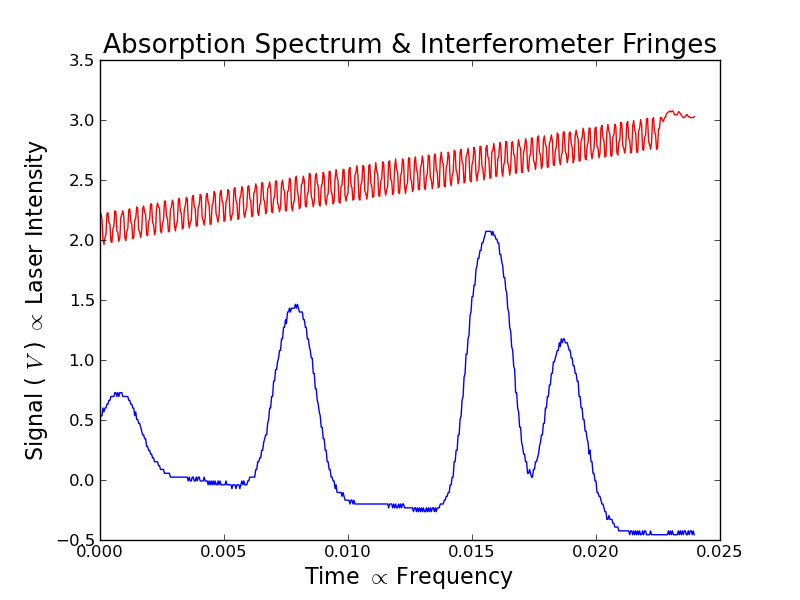
\includegraphics[height=70mm]{4-1-009.png}
  \caption{\textbf{Laser Intensity \& Interferometer Beam Intensity over Change in Frequency} demonstrating the changing intensity (fringes) generated by the interferometer over the same interval as the intensity incident from the laser beam traveling through the Rubidium chamber. }
  \label{fig:int_1}
\end{center} \end{figure}




%%%%%%%%%%%Results%%%%%%%%%%%%%%
\section{Results and Discussion}

Figures~\ref{fig:scaled_1}$-$\ref{fig:scaled_4} show four data samples illustrating hyperfine splitting plotted against frequency shift. In each of the plots, the first peak (corresponding to the 87a absorption) is denoted as the $\Delta 0.00$ GHz point. All subsequent shifts are relative to this initial peak. Values given on Tables~\ref{table:relativePositions87} and~\ref{table:relativePositions85} correspond to these numbers. Values given on these two tables were estimated, and in the case where an exact value was indeterminable, the field was left blank. Random error exists here both due to the time resolution with which the samples were taken and the human estimation.

\begin{figure}[H] \begin{center}
  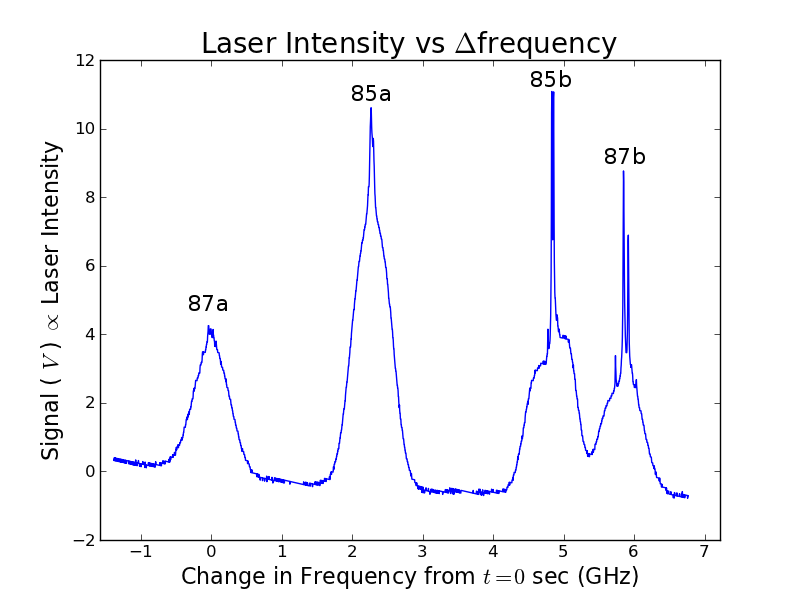
\includegraphics[height=70mm]{4-2-009.png}
  \caption{Saturated absorption \textbf{Plot of intensity vs. frequency shift} for data sample 1. }
  \label{fig:scaled_1}
\end{center} \end{figure}

\begin{figure}[H] \begin{center}
  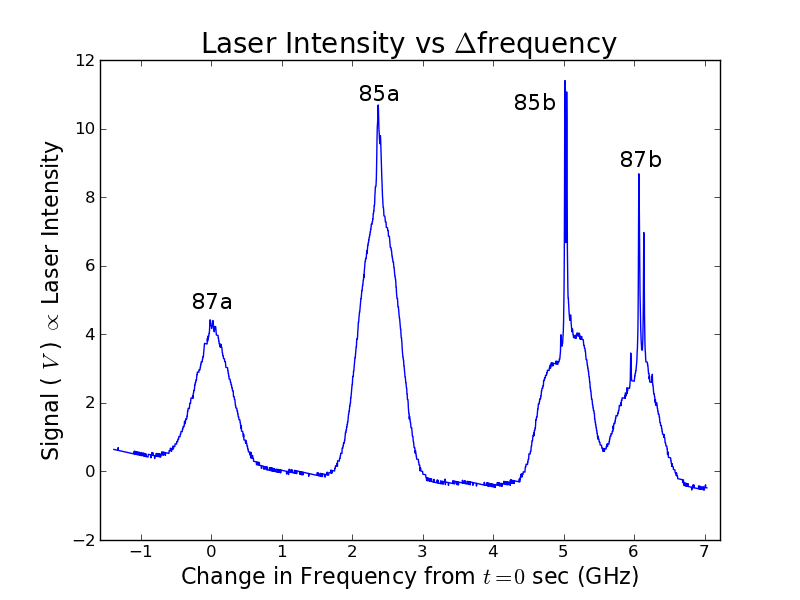
\includegraphics[height=60mm]{4-2-010.png}
  \caption{Saturated absorption \textbf{Plot of intensity vs. frequency shift} for data sample 2. }
  \label{fig:scaled_2}
\end{center} \end{figure}

\begin{figure}[H] \begin{center}
  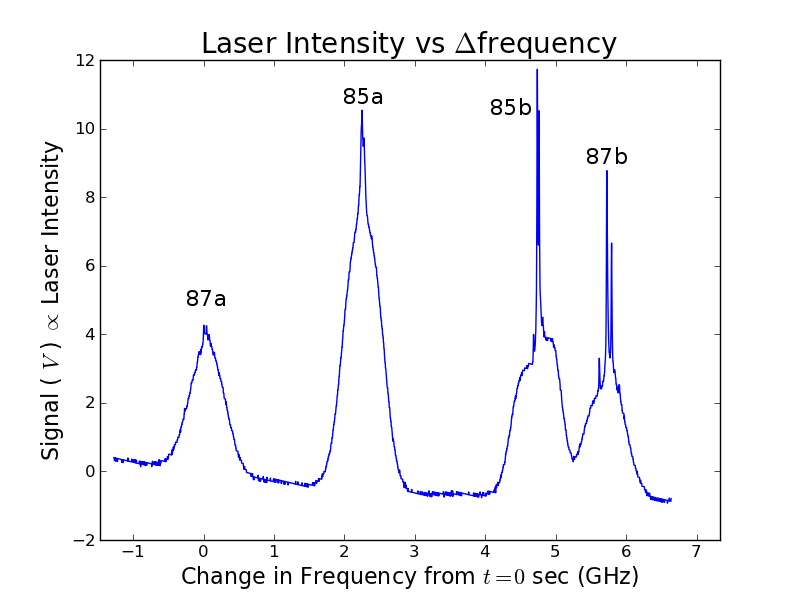
\includegraphics[height=60mm]{4-2-011.png}
  \caption{Saturated absorption \textbf{Plot of intensity vs. frequency shift} for data sample 3. }
  \label{fig:scaled_3}
\end{center} \end{figure}

\begin{figure}[H] \begin{center}
  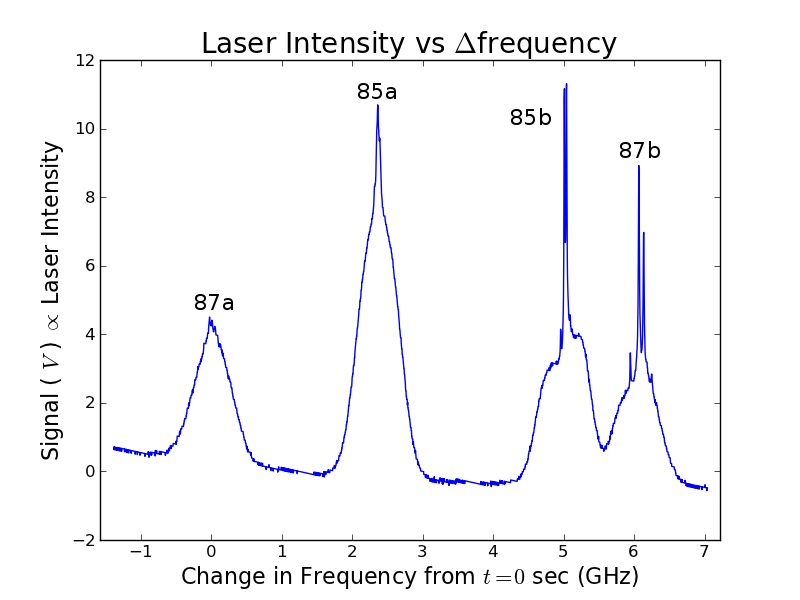
\includegraphics[height=60mm]{4-2-012.png}
  \caption{Saturated absorption \textbf{Plot of intensity vs. frequency shift}  for data sample 4. }
  \label{fig:scaled_4}
\end{center} \end{figure}

\begin{table}[H]
\centering
\caption{Relative positions of peaks (in GHz) for $^{87}$Rb, with values given to $\pm 0.05$ GHz}
\begin{tabular}{ c | c c c c | c c c c }
  \hline
  \hline
  sample no. & a & & & & b   \\
  \hline
  1 & $-$ & $-$ & $-$ & $-$ & 5.97 & 6.09 & 6.16 & 6.27 \\
  2 & 0.00 & 0.04 & 0.08 & $-$ & 5.97 & 6.09 & 6.16 & 6.28 \\
  3 & 0.00 & 0.04 & $-$ & $-$ & 5.62 & 5.73 & 5.79 & 5.83  \\
  4 & 0.00 & 0.03 & 0.07 & $-$ & 5.97 & 6.09 & 6.17 & 6.28
\end{tabular}
\label{table:relativePositions87}
\end{table}

\begin{table}[H]
\centering
\caption{Relative positions of peaks (in GHz) for $^{85}$Rb, with values given to $\pm 0.05$ GHz}
\begin{tabular}{ c | c c c c | c c c c | c c c c | c c c c }
  \hline
  \hline
  sample no. & a & & & & b  \\
  \hline
  1 & 2.5 & 2.53 & $-$ & $-$ & 5.01 & 5.07 & 5.10 & 5.15 \\
  2 & 2.39 & 2.42 & $-$ & $-$ & 4.98 & 5.04 & 5.06 & 5.12 \\
  3 & 2.25 & 2.27 & $-$ & $-$ & 4.68 & 4.74 & 4.76 & 4.81 \\
  4 & 2.34 & 2.39 & 2.42 & $-$ & 4.99 & 5.04 & 5.07 & 5.12 
\end{tabular}
\label{table:relativePositions85}
\end{table}

Average frequency offsets between groupings of peaks are given in Table~\ref{table:freqOffset} below.

\begin{table}[H]
\centering
\caption{Average frequency difference ($\Delta$GHz) between peaks with associated error}
\begin{tabular}{ || c | c c c c || }
  \hline
  \hline
   $-$ & 87a & 85a & 85b & 87b \\
  \hline
  87a & $-$ & $2.37 \pm 0.14$ & $4.97 \pm 0.23$ & $6.03 \pm 0.53$ \\
  85a & $2.37 \pm 0.14$ & $-$ & $2.60 \pm 0.13$ & $3.64 \pm 0.18$ \\
  85b & $4.97 \pm 0.23$ & $2.60 \pm 0.13$ & $-$ &  $1.04 \pm 0.07$ \\
  87b & $6.03 \pm 0.53$ & $3.64 \pm 0.18$ & $1.04 \pm 0.07$ & $-$  \\
  \hline
  \hline
\end{tabular}
\label{table:freqOffset}
\end{table}

\begin{figure*}[h]
  \centering
  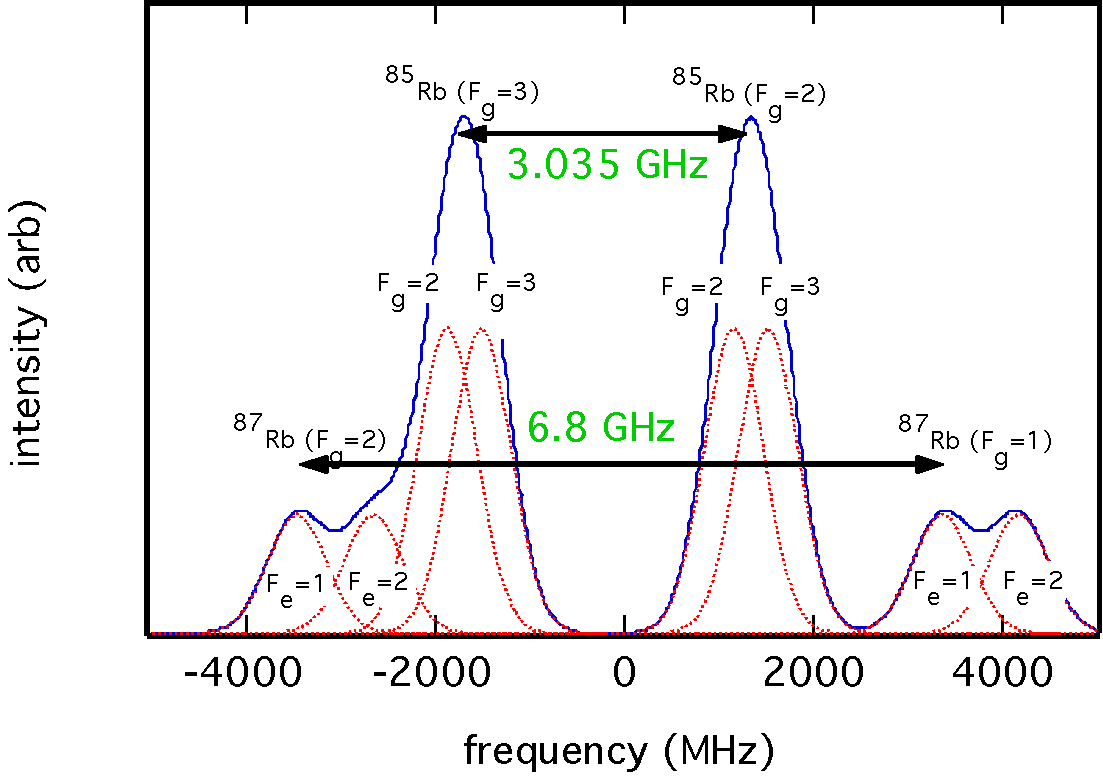
\includegraphics[width=3in]{/Users/adamreyes/Dropbox/AdvancedLab/Diode-Laser-Spec/WriteUp/figures_laserspec/fluorescence.png}
  \caption{Literature Values for the Rubidium absorption lines\cite{vanier}\cite{harvard}}
  \label{fig:literature}
\end{figure*}

Using the Michelson Interferometer we determined that for our settings
each $0.00020475s$ of the oscilloscope trace gives a change in
frequency of $0.08347 \pm 0.05$ GHz. Here, our error is in large part
dominated by our measurement of the path length difference of the two
arms of the interferometer. The relative magnitude of this error could
have been significantly decreased had we been able to get a larger
path length difference between the two arms. The main obstacle we
faced in trying to do so was that the BNC cable going to the detectors
were not long enough to reach the far side of the table, effectively
limiting the possible path length of the long arm. \\

Figure ~\ref{fig:literature} replots data from
\cite{vanier}. Specifically it shows the line spacing between the two
furthest lines (6.8 GHz) and the middle two lines (3.035 GHz). This is
somewhat comparable (though not entirely so) to our measured spectrum with spacings shown in Table~\ref{table:freqOffset}.

%% hey so we're not exactly on with these values, even with errors. is there anything you want to add here?

\vspace{3em}

Because there was extra time available at the end of the experiment, we decided to attempt to observe the relation between resonant absorption and the refractive index in Rb gas.

To do so, we took one incident beam, split it in two, passed one through the Rb chamber, and had the other travel the same distance, but not pass through the chamber. The two beams were then recombined and this sum (with interference) was then passed into a photoelectric diode. Changes in frequency between the two beams (frequency change due to refractive index of Rb gas) should effect interference which should be measurable with the diode.

Unfortunately, we were unable to precisely reproduce this effect. We attempted aligning the two beams multiple ways; however, we never were able to see evidence of interference, or if we did, it was too faint to be in any way noticeable.
% NOTE ABOVE THAT "EFFECT" with an "E" is the right word to use. I know the verb is normally "Affect", but in this case it's "effect". Not to be rude, just /so many people/ get this wrong because they learn that an "effect" is only ever a noun.




%%%%%%%%%%%%%References%%%%%%%%%%%%%%%%%%%%
\begin{thebibliography}{99}
\bibitem{vanier}Jacques Vanier. Relaxation in rubidium-87 and the
  rubidium maser. Phys. Rev., 168:129-149, 1968.
\bibitem{harvard}"Rubidium Fluoresence." Cfa.harvard.edu. Harvard, n.d. Web.
\end{thebibliography}


% %%%%%%%%%%%%%% Absorption figure%%%%%%%%%%%%%%%%%%
% \begin{figure}[h]
%   \centering
%   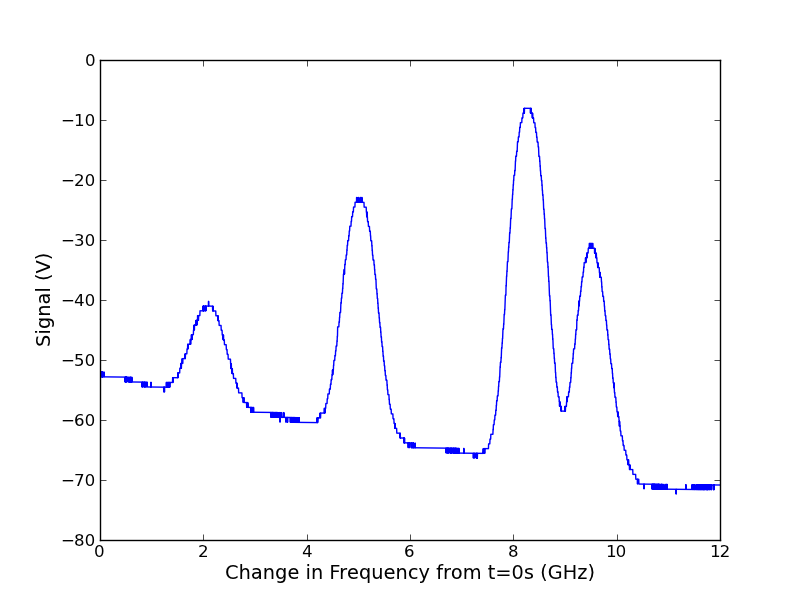
\includegraphics[width=3in]{/Users/adamreyes/Dropbox/AdvancedLab/Diode-Laser-Spec/WriteUp/figures_laserspec/ag-4-2-001_freq.png}
%   \caption{Measured Transmission Absorption Spectrum for Rubidium.}
%   \label{fig:absorption}
% \end{figure}
% %%%%%%%%%% 
% %%%%%%%%%%%%%%%%%% Saturated Absorption figure%%%%%%%%
% \begin{figure*}[h]
%   \centering
%   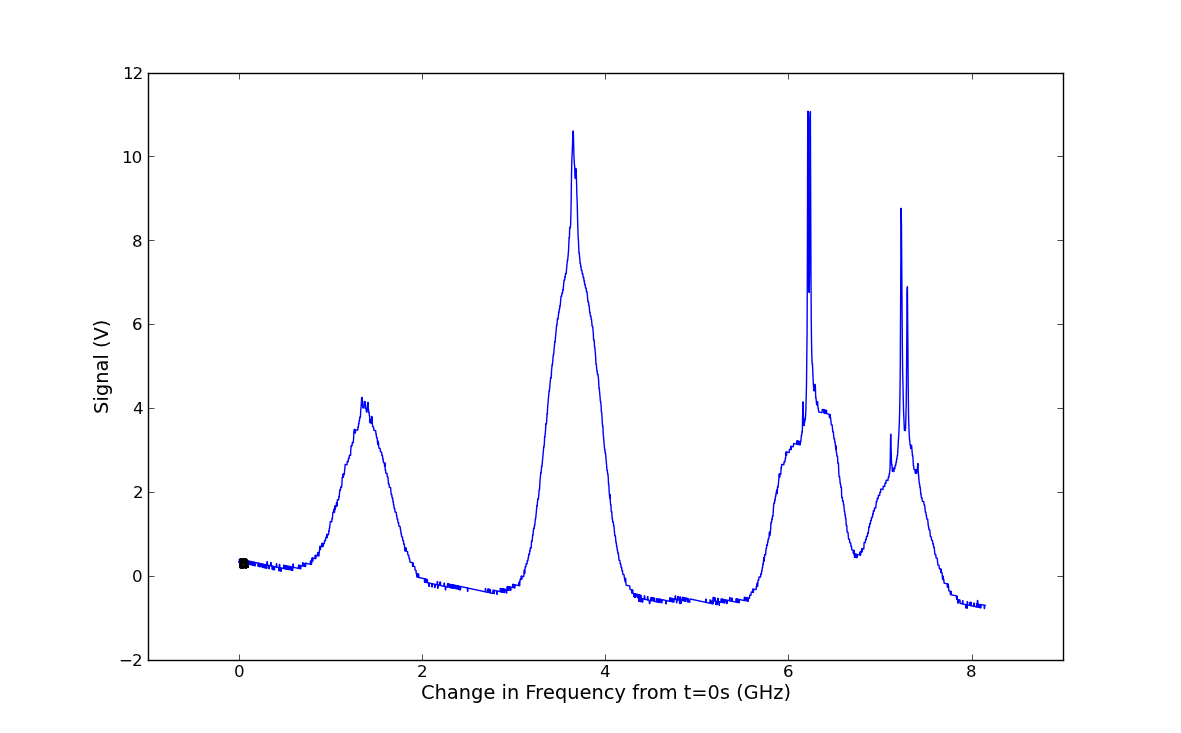
\includegraphics[width=3in]{/Users/adamreyes/Dropbox/AdvancedLab/Diode-Laser-Spec/WriteUp/figures_laserspec/ag-4-2-009_saturated.png}
%   \caption{Measured Saturated Absorption Spectrum for Rubidium with electronic subtration of doppler broadening and laser current modulation}
%   \label{fig:saturatedabsorption}
% \end{figure*}
% %%%%%%%%%% 


\end{document}